%\begin{frame}{titel}
%    \pause
%    \begin{columns}
%        \begin{column}{0.5\textwidth}
%            \begin{itemize}
%                \item <->
%                \item <->
%                \item <->
%                \item <->
%                \item <->
%                \item <->
%            \end{itemize}
%        \end{column}
%        \begin{column}{0.5\textwidth}
%            \centering
%            \only <->{
%                \includegraphics[scale=0.25]{images/}\\[-0.5\baselineskip]
%                \hspace{1.5cm}}%\href{www. ...}{[name, paper]}
%             }
%        \end{column}
%    \end{columns}
%\end{frame}


\section{Experimenteller Aufbau und Durchführung}
%\subsection{Experimenteller Aufbau}
%\begin{frame}{Experimenteller Aufbau}
%    \pause
%    \begin{columns}
%        \begin{column}{0.5\textwidth}
%            \begin{itemize}
%                \item <1-> Hauptbestandteile
%                \begin{itemize}
%                    \item <2-> Festkörperlaser (grün) $\lambda= \SI{552}{\nano\meter}$ 
%                    \item <3-> Probe 
%                    \item <4-> Spektrometer  
%                \end{itemize}
%                \item <5-> ebenfalls Bestandteile sind
%                \begin{itemize}
%                    \item <4-> Durchfluss-Kryostat, Spulenpaar ($B = \SI{0,5}{\tesla}$)
%                    \item <5-> Tief- und Langpass
%                    \item <6-> BSC, Mikroskop Objektiv, Spiegel, Linsen
%                    \item <7-> Glan Thompson Prisma, Kamera, $\lambda /2$-Plättchen
%                \end{itemize}
%            \end{itemize}                
%        \end{column}
%        \begin{column}{0.5\textwidth}
%            \centering
%            \only <2->{
%            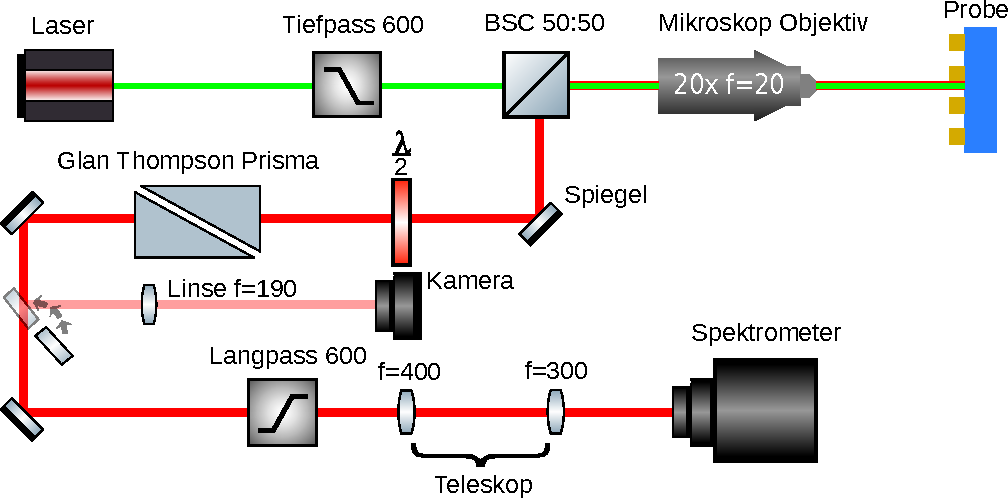
\includegraphics[scale=0.45]{images/setup.pdf}\\[-0.5\baselineskip]
%            }
%        \end{column}
%    \end{columns}
%\end{frame}


\begin{frame}{Experimenteller Aufbau}
    \pause
    \centering
    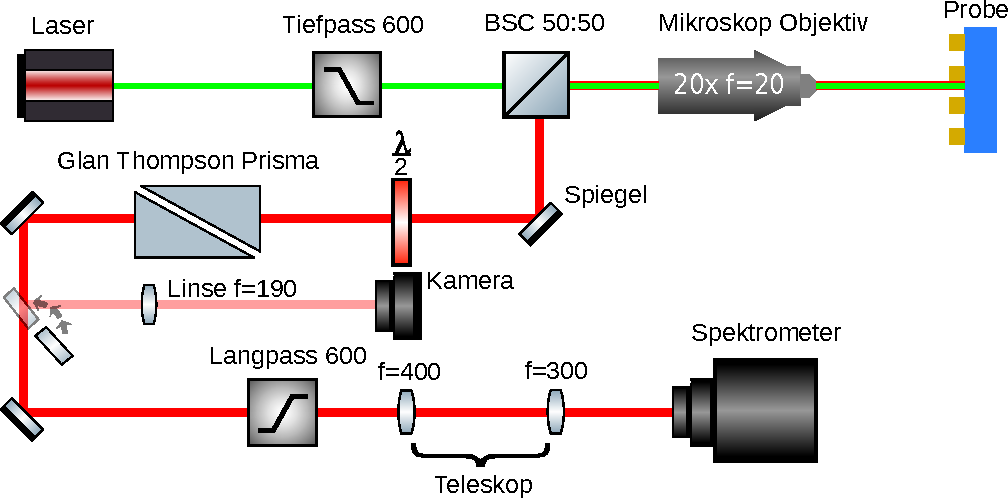
\includegraphics[scale=0.6]{images/setup.pdf}\\[-0.5\baselineskip]
\end{frame}


%\subsection{Experimentelle Durchführung}
\begin{frame}{Experimentelle Durchführung}
    \pause
    \begin{columns}
        \begin{column}{0.5\textwidth}
            \begin{itemize}
                \item <1-> Probe in den Fokus Mikroskopobjektivs 
                \bigskip
                \item <3-> Temperatureinstellung 
                    %\begin{itemize}
                    %    \item <4-> durch Heliumfluss und Heizelement
                    %\end{itemize}
                \bigskip
                \item <4-> Messung des Hintergrunds
                \bigskip
                \item <5-> abwechselndes aufnehmen von Spektren bei pos. und neg. Magnetfeld
                    %\begin{itemize}
                    %    \item <6-> 16 Einzelbildern mit jeweils 3 Sekunden Belichtungszeit, die aufaddiert werden
                    %    (Einzelbilder da sonst Sättigung der CCD)
                    %    \item <7->  insg. 26 Spektren bei pos. und neg. Magnetfeld
                    %    (Wechsel wirkt Störeffekten entgegen z.B. Änderungen der Laserintensität über Zeitraum)
                    %\end{itemize}
                \bigskip
                \item <6-> Nach Messung wird nächste Temperatur eingestellt
            \end{itemize}                
        \end{column}
        \begin{column}{0.5\textwidth}
            \centering
            %\only <2->{
            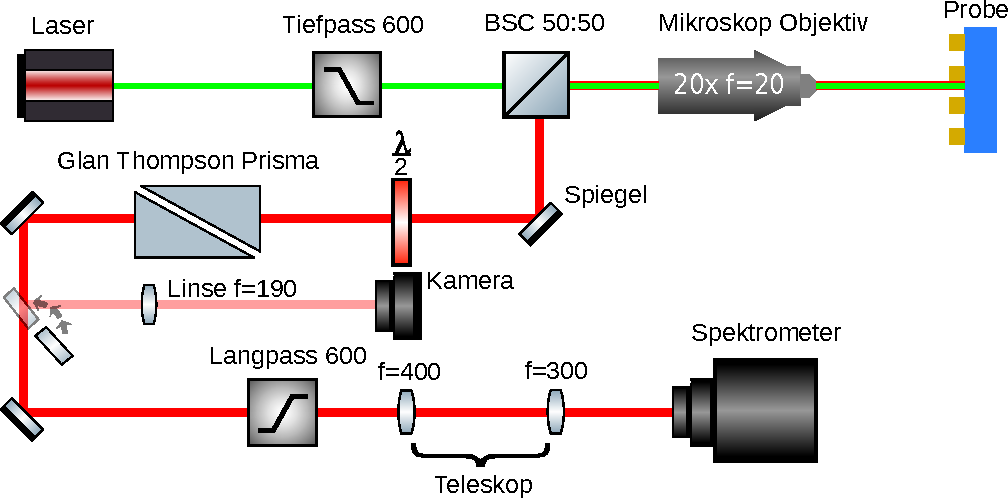
\includegraphics[scale=0.45]{images/setup.pdf}\\[-0.5\baselineskip]
            %}
        \end{column}
    \end{columns}
\end{frame}